\chapter{The way to get better results}
In this chapter described a way to improve genetic solver to solve more complex problems.
To do this, a benchmark measurement was made.
We concentrate on solving the problem with parameters:
\begin{itemize}
	\item variants: 10,
	\item depth: 2,
	\item requests: 15,
	\item resources: 5,
	\item timeout: 5 minutes.
\end{itemize}.
Due to the problem, the basic version of the genetic solver could not solve this problem at all. We do all this work to, firstly, achieve valid results, and then get a near-optimal solution. 
All measurements here and later were done at least five times. 
Figure~\ref{label} shown the box-plot of number of contract violation in basic version~\footnote{As a basic version taked version from 24.09.2019, commit: 57845c126c30a1ea59cb35eb16af0bd37930dda9} of genetic solver, as shown there are no valid results cause no results with zero contract violations.

\begin{figure}
	\centering
	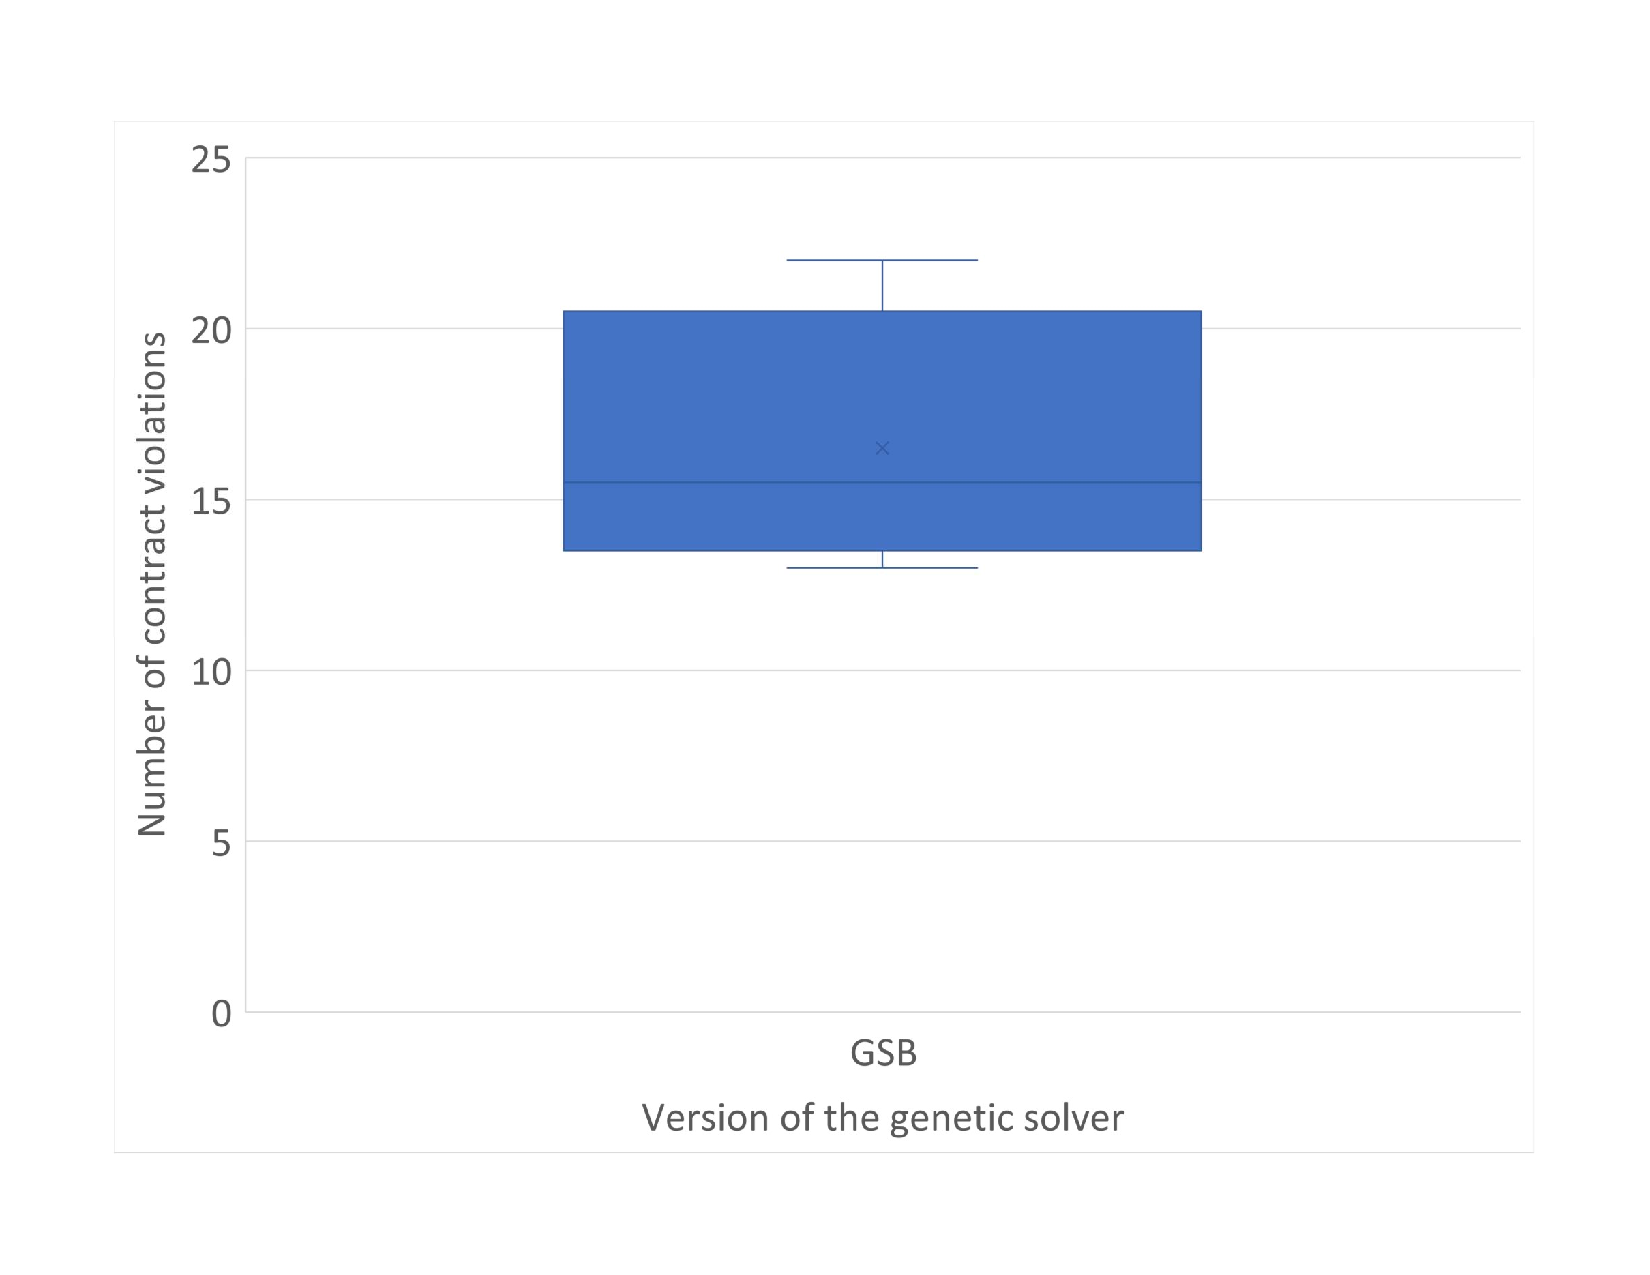
\includegraphics[width=\textwidth]{images/BoxPlotSolverBasic}
	\caption[Boxplot of number of contract violations for the basic version of genetic solver]{}
	\label{fig:boxplotsolverbasic}
\end{figure}


\section{Parameter tuning as a beginning of live}\todo{new title}
The first step to improve the genetic solver was a parameter optimization. To perform parameter optimization was performed a few important steps.
\begin{enumerate}
	\item Analysis of genetic solver to find out all parameters that could be changed. 
	\item Adapt BRISE to work with the genetic solver.
	\item Prepare Experiment description for BRISE.
	\item Run BRISE to get the optimal configuration.
\end{enumerate}

After deep-diving into the code of genetic solver, the list of parameters was prepared.
In the basic version of the genetic solver, there are only three parameters that are changeable on call. There are:
\begin{itemize}
	\item selectorType - type of the selector algorithm that was mentioned in section~\ref{sec:GeneticAlgorithm:Selector},
	\item number of generation - number of generations that performed by the genetic solver, working as a termination condition, in this thesis we use only timeout termination, so this parameter set as a huge value,
	\item PopulationSize - number of individuals in a population.
\end{itemize}

Adaptation of genetic solver to work into a BRISE consist of a few steps:
\begin{enumerate}
	\item prepare executable file of genetic solver,
	\item implement a method for a worker that will call the file from the previous step and returns the results with a number of contract violations and energy consumption.
\end{enumerate}

Step number 3 means that the user describes parameters that need to optimize, their names, ranges if the parameter has continuous range, or all variants if categorical. The user also should set what components to use, what the minimal number of measurements of a single Configuration, etc.
For parameter optimization of genetic solver, we use the experiment description shown in \todo{appendix or here?}.

When optimal configuration was founded, we use it to analyze results in a boxplot.
The results showed on Figure~\ref{fig:boxplotsolverbasictuning}.
\begin{figure}
	\centering
	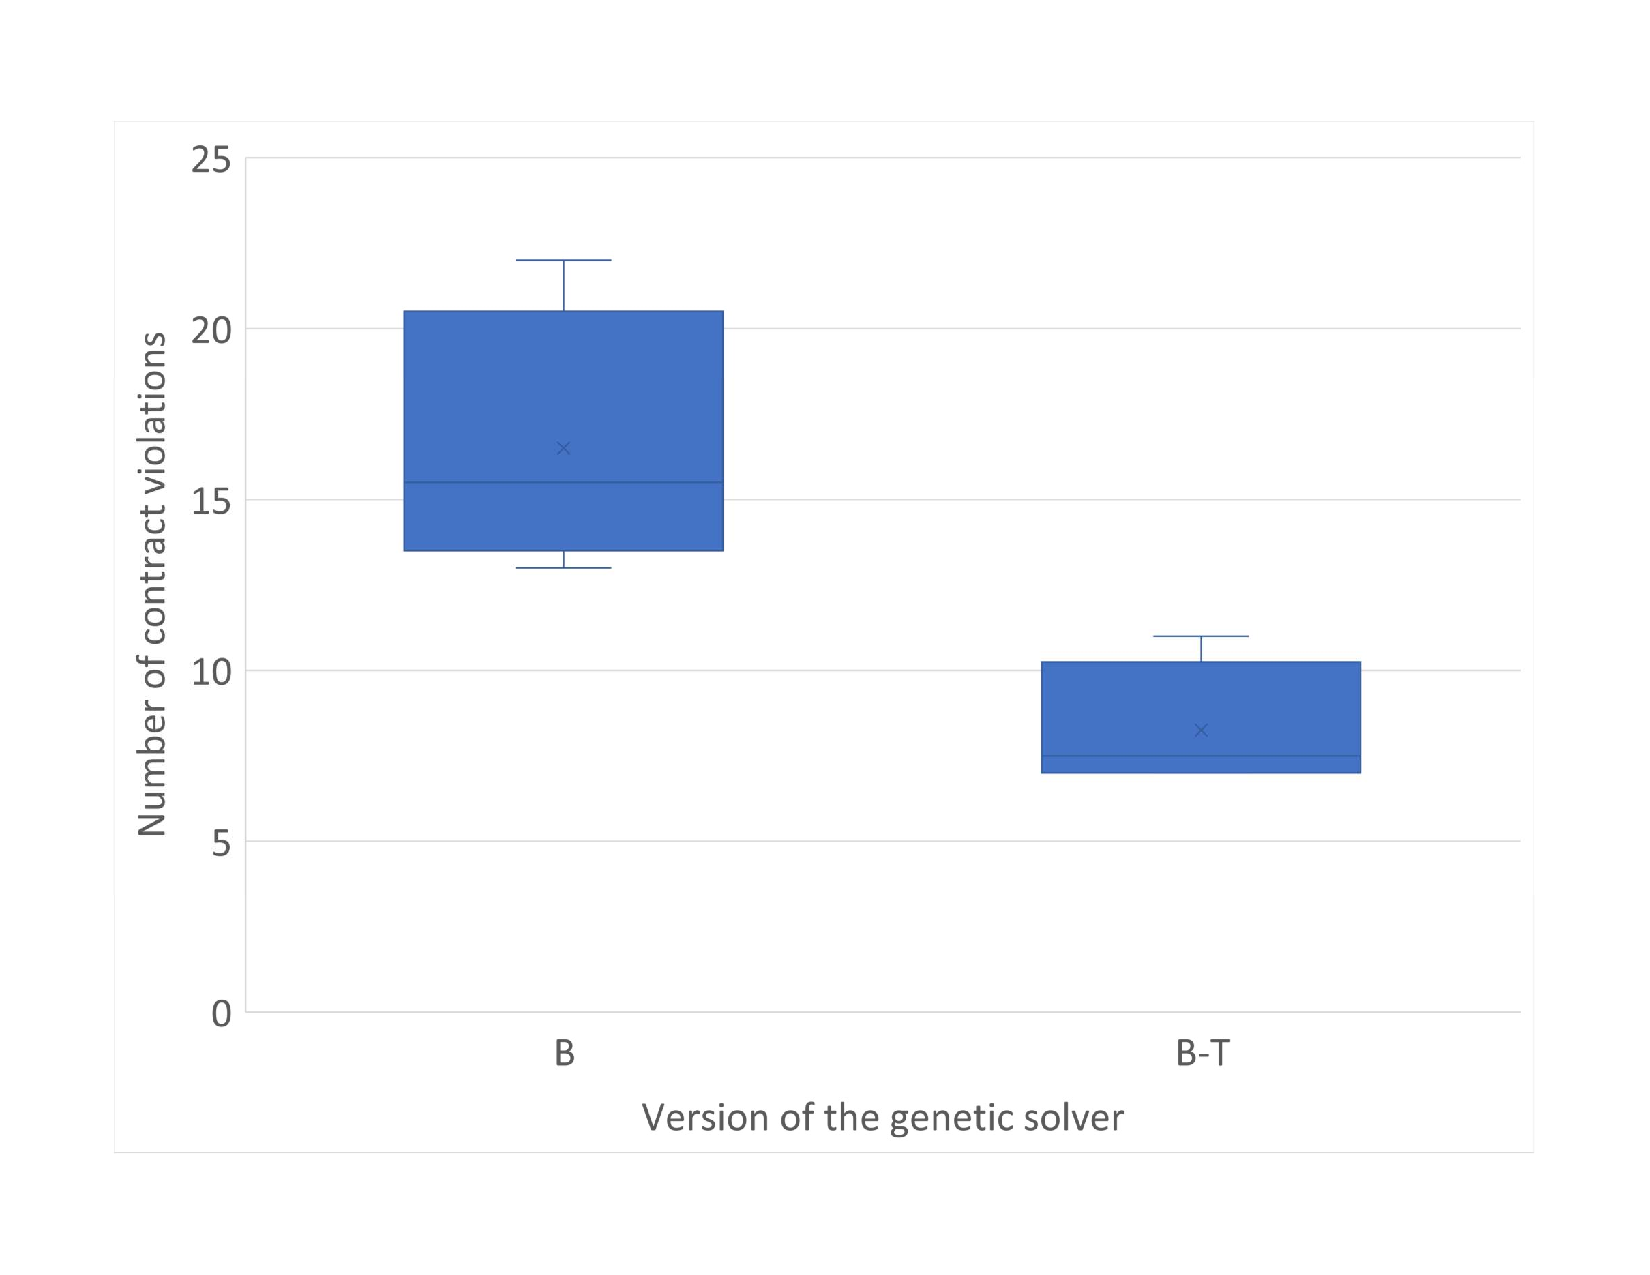
\includegraphics[width=\textwidth]{images/BoxPlotSolverBasicTuning}
	\caption[Boxplot of number of contract violations for the basic version of genetic solver and with tuned parameters]{}
	\label{fig:boxplotsolverbasictuning}
\end{figure}

Conclusions of this step:
\begin{enumerate}
	\item All results still not valid.
	\item Number of contract violations is less.
	\item The distance between max and min result is smaller.
	\item This step confirms the fact that good values of parameters have a big influence on the results, but sometimes parameter tuning not enough to get good results.
\end{enumerate}

\section{What if we could change magic numbers or Explain the code to ducks}
the section about how we replace the hardcoded parameters...

\section{Astrologers have announced a week of probabilities. The number of probabilities doubled.}
the section about new probabilities in Crossover and Mutation operators

\section{Rule34: optimize everything}
information how we optimize all parameters at this step

\section{Peppa Pig and adaptation for own life}
adaptive CrossoverRate and how it works

\section{Peppa Pig and life without cash as a result of optimal self-adaptation}
static tuning is good or not for adaptive parameters

\section{Unique genotypes is a God sign or placebo for genetic algorithms}
How works unique individuals in a population

\section{As my grandfather said: "I am your optimization"}
info about results of optimization

\section{Bermuda Triangle and Missing Parameters}
MAYBE there will be information about not important parameters

\section*{Conclusion - Today we dried coals using the oven in Aleksandrovka}
Combination of different techniques and optimizations could give you better results 